\documentclass[Rapport/Rapport_main.tex]{subfiles}
\begin{document}
\subsection{Grænseflader}\label{sec:rap_interfaces}
I dette afsnit beskrives, hvordan I2C protokollen mellem RPi'en(Master) og PSoC enhederne(slaves) anvendes. For den fulde dokumentation se \textbf{Arkitektur} \fullref{arch:sec:protocols}.
\subsubsection{Kommunikation mellem Rasberry Pi Zero W og PSoC enheder}
Playerside, BallDispenser og RPi enhederne er alle tilkoblet til samme I2C-bus. For I2C kommunikation gælder: 
\begin{itemize}
    \item Clock speed : 100 $\si{\frac{kbits}{s}}$ 
\end{itemize}
\textbf{Protokolstruktur}
\begin{figure}[H]
    \centering
    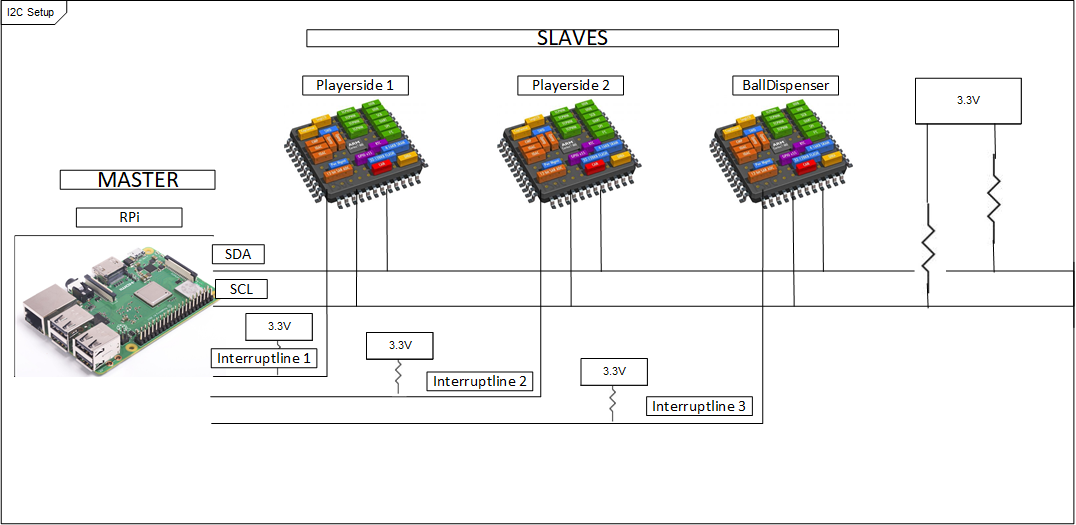
\includegraphics[width=\textwidth]{Rapport/Arkitektur/graphics/I2C-Illustration.png}
   \caption{Skitse af I2C kommunikation. Kommunikationen mellem enhederne starter enten med, at RPi'en(Master) ønsker at sende data til Playerside eller BallDispenser (Slaves), eller hvis en af slaverne trækker interruptlinjen lavt.}
    \label{fig:sketch_interrut}
\end{figure}

\subsubsection{Kommunikation mellem RPi og Playerside}
Playersides skal registere antal kopper tilbage på de angivne pladser. Denne information er vital for RPi’en, som videregiver denne information til Display. Playerside sender ét byte til RPi, hvor de 6 LSB repræsenterer en kop. Et højt bit betyder, at en kop er placeret på den angivne plads og et lavt bit betyder, at der ikke er en kop (Dette refereres fremover som 'cupstatus'), se figur \ref{fig:cups_setup}.
\begin{figure}[H]
    \centering
    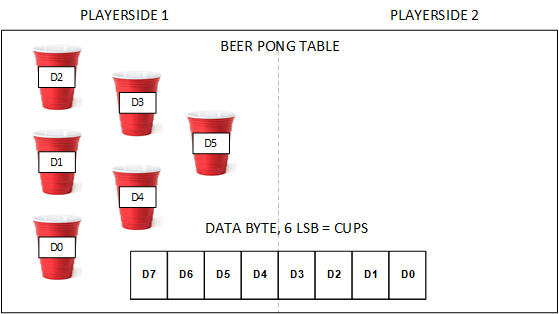
\includegraphics[width=\textwidth]{Arkitektur/Grenseflader/Graphics/cups.png}
    \caption{Repræsentation af 1 byte af kopper}
    \label{fig:cups_setup}
\end{figure}
\subsubsection{Kommunikation mellem RPi og BallDispenser}
RPi dikterer, hvilke tilstande BallDispenser-enheden skal instantiere, og BallDispenser sender hvilke events, som opstår for systemet: Ingen bolde eller Møntindkast.
\end{document}